\documentclass[]{article}
\usepackage{lmodern}
\usepackage{amssymb,amsmath}
\usepackage{ifxetex,ifluatex}
\usepackage{fixltx2e} % provides \textsubscript
\ifnum 0\ifxetex 1\fi\ifluatex 1\fi=0 % if pdftex
  \usepackage[T1]{fontenc}
  \usepackage[utf8]{inputenc}
\else % if luatex or xelatex
  \ifxetex
    \usepackage{mathspec}
  \else
    \usepackage{fontspec}
  \fi
  \defaultfontfeatures{Ligatures=TeX,Scale=MatchLowercase}
\fi
% use upquote if available, for straight quotes in verbatim environments
\IfFileExists{upquote.sty}{\usepackage{upquote}}{}
% use microtype if available
\IfFileExists{microtype.sty}{%
\usepackage{microtype}
\UseMicrotypeSet[protrusion]{basicmath} % disable protrusion for tt fonts
}{}
\usepackage[margin=1in]{geometry}
\usepackage{hyperref}
\hypersetup{unicode=true,
            pdftitle={PA1\_Template},
            pdfauthor={Jigar Patel},
            pdfborder={0 0 0},
            breaklinks=true}
\urlstyle{same}  % don't use monospace font for urls
\usepackage{color}
\usepackage{fancyvrb}
\newcommand{\VerbBar}{|}
\newcommand{\VERB}{\Verb[commandchars=\\\{\}]}
\DefineVerbatimEnvironment{Highlighting}{Verbatim}{commandchars=\\\{\}}
% Add ',fontsize=\small' for more characters per line
\usepackage{framed}
\definecolor{shadecolor}{RGB}{248,248,248}
\newenvironment{Shaded}{\begin{snugshade}}{\end{snugshade}}
\newcommand{\KeywordTok}[1]{\textcolor[rgb]{0.13,0.29,0.53}{\textbf{#1}}}
\newcommand{\DataTypeTok}[1]{\textcolor[rgb]{0.13,0.29,0.53}{#1}}
\newcommand{\DecValTok}[1]{\textcolor[rgb]{0.00,0.00,0.81}{#1}}
\newcommand{\BaseNTok}[1]{\textcolor[rgb]{0.00,0.00,0.81}{#1}}
\newcommand{\FloatTok}[1]{\textcolor[rgb]{0.00,0.00,0.81}{#1}}
\newcommand{\ConstantTok}[1]{\textcolor[rgb]{0.00,0.00,0.00}{#1}}
\newcommand{\CharTok}[1]{\textcolor[rgb]{0.31,0.60,0.02}{#1}}
\newcommand{\SpecialCharTok}[1]{\textcolor[rgb]{0.00,0.00,0.00}{#1}}
\newcommand{\StringTok}[1]{\textcolor[rgb]{0.31,0.60,0.02}{#1}}
\newcommand{\VerbatimStringTok}[1]{\textcolor[rgb]{0.31,0.60,0.02}{#1}}
\newcommand{\SpecialStringTok}[1]{\textcolor[rgb]{0.31,0.60,0.02}{#1}}
\newcommand{\ImportTok}[1]{#1}
\newcommand{\CommentTok}[1]{\textcolor[rgb]{0.56,0.35,0.01}{\textit{#1}}}
\newcommand{\DocumentationTok}[1]{\textcolor[rgb]{0.56,0.35,0.01}{\textbf{\textit{#1}}}}
\newcommand{\AnnotationTok}[1]{\textcolor[rgb]{0.56,0.35,0.01}{\textbf{\textit{#1}}}}
\newcommand{\CommentVarTok}[1]{\textcolor[rgb]{0.56,0.35,0.01}{\textbf{\textit{#1}}}}
\newcommand{\OtherTok}[1]{\textcolor[rgb]{0.56,0.35,0.01}{#1}}
\newcommand{\FunctionTok}[1]{\textcolor[rgb]{0.00,0.00,0.00}{#1}}
\newcommand{\VariableTok}[1]{\textcolor[rgb]{0.00,0.00,0.00}{#1}}
\newcommand{\ControlFlowTok}[1]{\textcolor[rgb]{0.13,0.29,0.53}{\textbf{#1}}}
\newcommand{\OperatorTok}[1]{\textcolor[rgb]{0.81,0.36,0.00}{\textbf{#1}}}
\newcommand{\BuiltInTok}[1]{#1}
\newcommand{\ExtensionTok}[1]{#1}
\newcommand{\PreprocessorTok}[1]{\textcolor[rgb]{0.56,0.35,0.01}{\textit{#1}}}
\newcommand{\AttributeTok}[1]{\textcolor[rgb]{0.77,0.63,0.00}{#1}}
\newcommand{\RegionMarkerTok}[1]{#1}
\newcommand{\InformationTok}[1]{\textcolor[rgb]{0.56,0.35,0.01}{\textbf{\textit{#1}}}}
\newcommand{\WarningTok}[1]{\textcolor[rgb]{0.56,0.35,0.01}{\textbf{\textit{#1}}}}
\newcommand{\AlertTok}[1]{\textcolor[rgb]{0.94,0.16,0.16}{#1}}
\newcommand{\ErrorTok}[1]{\textcolor[rgb]{0.64,0.00,0.00}{\textbf{#1}}}
\newcommand{\NormalTok}[1]{#1}
\usepackage{graphicx,grffile}
\makeatletter
\def\maxwidth{\ifdim\Gin@nat@width>\linewidth\linewidth\else\Gin@nat@width\fi}
\def\maxheight{\ifdim\Gin@nat@height>\textheight\textheight\else\Gin@nat@height\fi}
\makeatother
% Scale images if necessary, so that they will not overflow the page
% margins by default, and it is still possible to overwrite the defaults
% using explicit options in \includegraphics[width, height, ...]{}
\setkeys{Gin}{width=\maxwidth,height=\maxheight,keepaspectratio}
\IfFileExists{parskip.sty}{%
\usepackage{parskip}
}{% else
\setlength{\parindent}{0pt}
\setlength{\parskip}{6pt plus 2pt minus 1pt}
}
\setlength{\emergencystretch}{3em}  % prevent overfull lines
\providecommand{\tightlist}{%
  \setlength{\itemsep}{0pt}\setlength{\parskip}{0pt}}
\setcounter{secnumdepth}{0}
% Redefines (sub)paragraphs to behave more like sections
\ifx\paragraph\undefined\else
\let\oldparagraph\paragraph
\renewcommand{\paragraph}[1]{\oldparagraph{#1}\mbox{}}
\fi
\ifx\subparagraph\undefined\else
\let\oldsubparagraph\subparagraph
\renewcommand{\subparagraph}[1]{\oldsubparagraph{#1}\mbox{}}
\fi

%%% Use protect on footnotes to avoid problems with footnotes in titles
\let\rmarkdownfootnote\footnote%
\def\footnote{\protect\rmarkdownfootnote}

%%% Change title format to be more compact
\usepackage{titling}

% Create subtitle command for use in maketitle
\newcommand{\subtitle}[1]{
  \posttitle{
    \begin{center}\large#1\end{center}
    }
}

\setlength{\droptitle}{-2em}

  \title{PA1\_Template}
    \pretitle{\vspace{\droptitle}\centering\huge}
  \posttitle{\par}
    \author{Jigar Patel}
    \preauthor{\centering\large\emph}
  \postauthor{\par}
      \predate{\centering\large\emph}
  \postdate{\par}
    \date{December 8, 2018}


\begin{document}
\maketitle

\section{Reproducible Research}\label{reproducible-research}

Loading packages :

\begin{Shaded}
\begin{Highlighting}[]
  \KeywordTok{library}\NormalTok{(}\StringTok{"dplyr"}\NormalTok{)}
\end{Highlighting}
\end{Shaded}

\begin{verbatim}
## 
## Attaching package: 'dplyr'
\end{verbatim}

\begin{verbatim}
## The following objects are masked from 'package:stats':
## 
##     filter, lag
\end{verbatim}

\begin{verbatim}
## The following objects are masked from 'package:base':
## 
##     intersect, setdiff, setequal, union
\end{verbatim}

\begin{Shaded}
\begin{Highlighting}[]
  \KeywordTok{library}\NormalTok{(}\StringTok{"lubridate"}\NormalTok{)}
\end{Highlighting}
\end{Shaded}

\begin{verbatim}
## 
## Attaching package: 'lubridate'
\end{verbatim}

\begin{verbatim}
## The following object is masked from 'package:base':
## 
##     date
\end{verbatim}

\begin{Shaded}
\begin{Highlighting}[]
  \KeywordTok{library}\NormalTok{(}\StringTok{"data.table"}\NormalTok{)}
\end{Highlighting}
\end{Shaded}

\begin{verbatim}
## 
## Attaching package: 'data.table'
\end{verbatim}

\begin{verbatim}
## The following objects are masked from 'package:lubridate':
## 
##     hour, isoweek, mday, minute, month, quarter, second, wday,
##     week, yday, year
\end{verbatim}

\begin{verbatim}
## The following objects are masked from 'package:dplyr':
## 
##     between, first, last
\end{verbatim}

\begin{Shaded}
\begin{Highlighting}[]
  \KeywordTok{library}\NormalTok{(}\StringTok{"tibble"}\NormalTok{)}
  \KeywordTok{library}\NormalTok{(}\StringTok{"ggplot2"}\NormalTok{)}
  \KeywordTok{library}\NormalTok{(}\StringTok{"lattice"}\NormalTok{)}
\end{Highlighting}
\end{Shaded}

\begin{enumerate}
\def\labelenumi{\arabic{enumi}.}
\tightlist
\item
  reading the data file using fread and tbl\_df, also cleaning up the
  date column simultaneously using mutate
\end{enumerate}

\begin{Shaded}
\begin{Highlighting}[]
\NormalTok{    rawdata<-}\StringTok{ }\KeywordTok{tbl_df}\NormalTok{(}\KeywordTok{fread}\NormalTok{(}\StringTok{"activity.csv"}\NormalTok{, }\DataTypeTok{na.strings =} \StringTok{"NA"}\NormalTok{) ) }\OperatorTok\StringTok{  }\KeywordTok{mutate}\NormalTok{(}\DataTypeTok{date =} \KeywordTok{ymd}\NormalTok{(date))}
\end{Highlighting}
\end{Shaded}

\begin{enumerate}
\def\labelenumi{\arabic{enumi}.}
\setcounter{enumi}{1}
\tightlist
\item
  filtering out NA values
\end{enumerate}

\begin{Shaded}
\begin{Highlighting}[]
\NormalTok{    data <-}\StringTok{ }\KeywordTok{filter}\NormalTok{(rawdata, steps }\OperatorTok{!=}\StringTok{ 'NA'}\NormalTok{)}
\end{Highlighting}
\end{Shaded}

\begin{enumerate}
\def\labelenumi{\arabic{enumi}.}
\setcounter{enumi}{2}
\tightlist
\item
  aggregating data to get total steps each day
\end{enumerate}

\begin{Shaded}
\begin{Highlighting}[]
\NormalTok{  aggregated_totalsteps <-}\StringTok{ }\KeywordTok{aggregate}\NormalTok{(}\DataTypeTok{x =}\NormalTok{data[}\KeywordTok{c}\NormalTok{(}\StringTok{"steps"}\NormalTok{,}\StringTok{"interval"}\NormalTok{)], }\DataTypeTok{by =} \KeywordTok{list}\NormalTok{(data}\OperatorTok{$}\NormalTok{date),}\DataTypeTok{FUN =}\NormalTok{ sum)}
\end{Highlighting}
\end{Shaded}

\begin{enumerate}
\def\labelenumi{\arabic{enumi}.}
\setcounter{enumi}{3}
\tightlist
\item
  creating histogram of total steps per day using qplot
\end{enumerate}

\begin{Shaded}
\begin{Highlighting}[]
\KeywordTok{qplot}\NormalTok{(aggregated_totalsteps}\OperatorTok{$}\NormalTok{steps, }\DataTypeTok{geom=}\StringTok{"histogram"}\NormalTok{,}\DataTypeTok{binwidth=} \DecValTok{5000}\NormalTok{, }\DataTypeTok{main =} \StringTok{"Histogram for Steps"}\NormalTok{, }\DataTypeTok{xlab =} \StringTok{"Total Steps Per Day"}\NormalTok{)}
\end{Highlighting}
\end{Shaded}

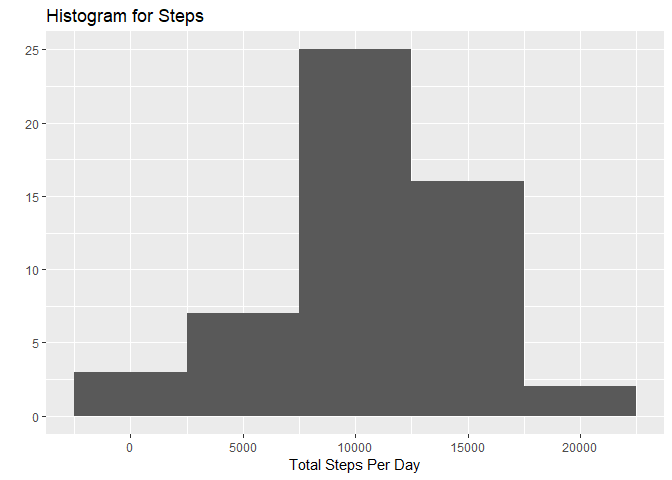
\includegraphics{PA1_template_files/figure-latex/unnamed-chunk-5-1.pdf}

\begin{enumerate}
\def\labelenumi{\arabic{enumi}.}
\setcounter{enumi}{4}
\tightlist
\item
  mean steps
\end{enumerate}

\begin{Shaded}
\begin{Highlighting}[]
\NormalTok{Meansteps <-}\StringTok{ }\KeywordTok{mean}\NormalTok{(aggregated_totalsteps}\OperatorTok{$}\NormalTok{steps)}
\end{Highlighting}
\end{Shaded}

\begin{enumerate}
\def\labelenumi{\arabic{enumi}.}
\setcounter{enumi}{5}
\tightlist
\item
  median steps
\end{enumerate}

\begin{Shaded}
\begin{Highlighting}[]
\NormalTok{Mediansteps <-}\StringTok{ }\KeywordTok{median}\NormalTok{(aggregated_totalsteps}\OperatorTok{$}\NormalTok{steps)}
\end{Highlighting}
\end{Shaded}

\subsection{What is the average daily activity
pattern?}\label{what-is-the-average-daily-activity-pattern}

\begin{enumerate}
\def\labelenumi{\arabic{enumi}.}
\setcounter{enumi}{6}
\tightlist
\item
  aggregrating data by interval for time series plot
\end{enumerate}

\begin{Shaded}
\begin{Highlighting}[]
\NormalTok{Byinterval <-}\StringTok{ }\KeywordTok{aggregate}\NormalTok{(data}\OperatorTok{$}\NormalTok{steps, }\DataTypeTok{by =} \KeywordTok{list}\NormalTok{(data}\OperatorTok{$}\NormalTok{interval), mean)}
\KeywordTok{colnames}\NormalTok{(Byinterval)<-}\KeywordTok{c}\NormalTok{(}\StringTok{"intervalID"}\NormalTok{, }\StringTok{"Mean steps"}\NormalTok{)}
\end{Highlighting}
\end{Shaded}

\begin{enumerate}
\def\labelenumi{\arabic{enumi}.}
\setcounter{enumi}{7}
\tightlist
\item
  Time Series plot
\end{enumerate}

\begin{Shaded}
\begin{Highlighting}[]
\KeywordTok{plot}\NormalTok{(Byinterval}\OperatorTok{$}\NormalTok{intervalID,Byinterval}\OperatorTok{$}\StringTok{`}\DataTypeTok{Mean steps}\StringTok{`}\NormalTok{,}\DataTypeTok{type=}\StringTok{"l"}\NormalTok{,}\DataTypeTok{xlab=}\StringTok{"5-Minute Interval"}\NormalTok{,}\DataTypeTok{ylab=}\StringTok{"Mean Steps Taken"}\NormalTok{,}
     
     \DataTypeTok{main=}\StringTok{"Steps during the Day"}\NormalTok{)}
\end{Highlighting}
\end{Shaded}

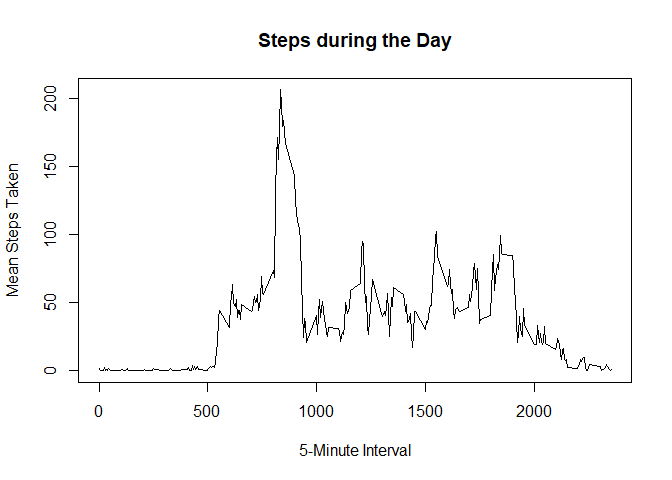
\includegraphics{PA1_template_files/figure-latex/unnamed-chunk-9-1.pdf}

\begin{enumerate}
\def\labelenumi{\arabic{enumi}.}
\setcounter{enumi}{8}
\tightlist
\item
  Interval with most activity
\end{enumerate}

\begin{Shaded}
\begin{Highlighting}[]
\NormalTok{Byinterval}\OperatorTok{$}\NormalTok{intervalID[}\KeywordTok{which.max}\NormalTok{(Byinterval}\OperatorTok{$}\StringTok{`}\DataTypeTok{Mean steps}\StringTok{`}\NormalTok{)]}
\end{Highlighting}
\end{Shaded}

\begin{verbatim}
## [1] 835
\end{verbatim}

\subsection{Imputing missing values}\label{imputing-missing-values}

\begin{enumerate}
\def\labelenumi{\arabic{enumi}.}
\setcounter{enumi}{9}
\tightlist
\item
  Let us re-read the raw data
\end{enumerate}

\begin{Shaded}
\begin{Highlighting}[]
\NormalTok{data2<-}\StringTok{ }\KeywordTok{tbl_df}\NormalTok{(}\KeywordTok{fread}\NormalTok{(}\StringTok{"activity.csv"}\NormalTok{, }\DataTypeTok{na.strings =} \StringTok{"NA"}\NormalTok{) ) }\OperatorTok\StringTok{  }\KeywordTok{mutate}\NormalTok{(}\DataTypeTok{date =} \KeywordTok{ymd}\NormalTok{(date))}
\end{Highlighting}
\end{Shaded}

\begin{enumerate}
\def\labelenumi{\arabic{enumi}.}
\setcounter{enumi}{10}
\tightlist
\item
  How many missing values
\end{enumerate}

\begin{Shaded}
\begin{Highlighting}[]
\KeywordTok{sum}\NormalTok{(}\OperatorTok{!}\KeywordTok{complete.cases}\NormalTok{(data2))}
\end{Highlighting}
\end{Shaded}

\begin{verbatim}
## [1] 2304
\end{verbatim}

\begin{enumerate}
\def\labelenumi{\arabic{enumi}.}
\setcounter{enumi}{11}
\tightlist
\item
  Replacing missing values with mean from that specific interval (Ex:
  Missing value in interval 5 replaced by mean step value in interval 5
\end{enumerate}

\begin{Shaded}
\begin{Highlighting}[]
\NormalTok{summary <-}\StringTok{ }\NormalTok{data2[}\KeywordTok{complete.cases}\NormalTok{(data2), ] }\OperatorTok\StringTok{ }\KeywordTok{group_by}\NormalTok{(interval) }\OperatorTok\StringTok{ }\KeywordTok{summarise}\NormalTok{(}\DataTypeTok{mean=}\KeywordTok{mean}\NormalTok{(steps));}
\NormalTok{incomplete <-}\StringTok{ }\NormalTok{data2[}\OperatorTok{!}\KeywordTok{complete.cases}\NormalTok{(data2),];}
\NormalTok{updated <-}\StringTok{ }\KeywordTok{merge}\NormalTok{(}\DataTypeTok{x=}\NormalTok{incomplete, }\DataTypeTok{y=}\NormalTok{summary, }\DataTypeTok{by=}\StringTok{"interval"}\NormalTok{, }\DataTypeTok{all.x=}\NormalTok{T);}
\NormalTok{updated}\OperatorTok{$}\NormalTok{steps <-}\StringTok{ }\NormalTok{updated}\OperatorTok{$}\NormalTok{mean;}
\NormalTok{imputed <-}\StringTok{ }\KeywordTok{rbind}\NormalTok{(data2[}\KeywordTok{complete.cases}\NormalTok{(data2), ], }\KeywordTok{select}\NormalTok{(updated, steps, date, interval))}
\end{Highlighting}
\end{Shaded}

\begin{enumerate}
\def\labelenumi{\arabic{enumi}.}
\setcounter{enumi}{12}
\tightlist
\item
  no more NA values
\end{enumerate}

\begin{Shaded}
\begin{Highlighting}[]
\KeywordTok{sum}\NormalTok{(}\OperatorTok{!}\KeywordTok{complete.cases}\NormalTok{(imputed))}
\end{Highlighting}
\end{Shaded}

\begin{verbatim}
## [1] 0
\end{verbatim}

\begin{enumerate}
\def\labelenumi{\arabic{enumi}.}
\setcounter{enumi}{13}
\tightlist
\item
  aggregating data2 to get total steps each day
\end{enumerate}

\begin{Shaded}
\begin{Highlighting}[]
\NormalTok{aggregated_totalsteps2 <-}\StringTok{ }\KeywordTok{aggregate}\NormalTok{(}\DataTypeTok{x =}\NormalTok{imputed[}\KeywordTok{c}\NormalTok{(}\StringTok{"steps"}\NormalTok{,}\StringTok{"interval"}\NormalTok{)], }\DataTypeTok{by =} \KeywordTok{list}\NormalTok{(imputed}\OperatorTok{$}\NormalTok{date),}\DataTypeTok{FUN =}\NormalTok{ sum)}
\end{Highlighting}
\end{Shaded}

\begin{enumerate}
\def\labelenumi{\arabic{enumi}.}
\setcounter{enumi}{14}
\tightlist
\item
  creating the new histogram of total steps per day using qplot
\end{enumerate}

\begin{Shaded}
\begin{Highlighting}[]
\KeywordTok{qplot}\NormalTok{(aggregated_totalsteps2}\OperatorTok{$}\NormalTok{steps, }\DataTypeTok{geom=}\StringTok{"histogram"}\NormalTok{,}\DataTypeTok{binwidth=} \DecValTok{5000}\NormalTok{, }\DataTypeTok{main =} \StringTok{"Histogram for Steps"}\NormalTok{, }\DataTypeTok{xlab =} \StringTok{"Total Steps Per Day"}\NormalTok{)}
\end{Highlighting}
\end{Shaded}

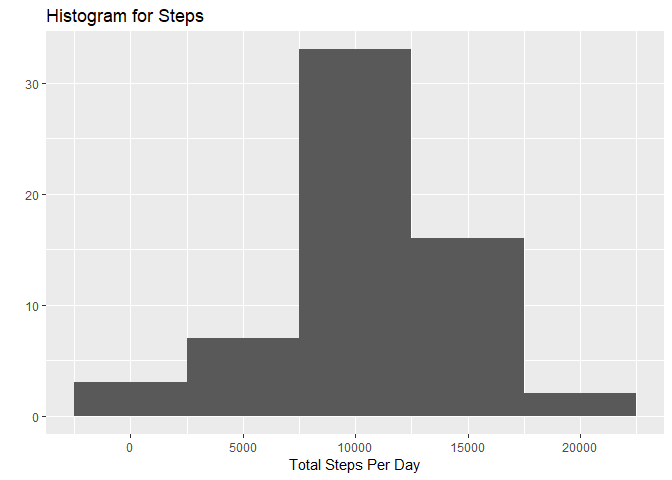
\includegraphics{PA1_template_files/figure-latex/unnamed-chunk-16-1.pdf}

\begin{enumerate}
\def\labelenumi{\arabic{enumi}.}
\setcounter{enumi}{15}
\tightlist
\item
  new mean steps
\end{enumerate}

\begin{Shaded}
\begin{Highlighting}[]
\NormalTok{Meansteps2 <-}\StringTok{ }\KeywordTok{mean}\NormalTok{(aggregated_totalsteps2}\OperatorTok{$}\NormalTok{steps)}
\end{Highlighting}
\end{Shaded}

\begin{enumerate}
\def\labelenumi{\arabic{enumi}.}
\setcounter{enumi}{16}
\tightlist
\item
  median steps
\end{enumerate}

\begin{Shaded}
\begin{Highlighting}[]
\NormalTok{Mediansteps2 <-}\StringTok{ }\KeywordTok{median}\NormalTok{(aggregated_totalsteps2}\OperatorTok{$}\NormalTok{steps)}
\end{Highlighting}
\end{Shaded}

\subsection{Are there differences in activity patterns between weekdays
and
weekends?}\label{are-there-differences-in-activity-patterns-between-weekdays-and-weekends}

\begin{enumerate}
\def\labelenumi{\arabic{enumi}.}
\setcounter{enumi}{17}
\tightlist
\item
  Creating a new column that classifies date column into weekend/weekday
\end{enumerate}

\begin{Shaded}
\begin{Highlighting}[]
\NormalTok{imputed}\OperatorTok{$}\NormalTok{day<-}\KeywordTok{ifelse}\NormalTok{(}\KeywordTok{as.POSIXlt}\NormalTok{(}\KeywordTok{as.Date}\NormalTok{(imputed}\OperatorTok{$}\NormalTok{date))}\OperatorTok{$}\NormalTok{wday}\OperatorTok\DecValTok{6}\OperatorTok{==}\DecValTok{0}\NormalTok{,}
                         \StringTok{"weekend"}\NormalTok{,}\StringTok{"weekday"}\NormalTok{)}

\NormalTok{imputed}\OperatorTok{$}\NormalTok{day<-}\KeywordTok{factor}\NormalTok{(imputed}\OperatorTok{$}\NormalTok{day,}\DataTypeTok{levels=}\KeywordTok{c}\NormalTok{(}\StringTok{"weekday"}\NormalTok{,}\StringTok{"weekend"}\NormalTok{))}
\end{Highlighting}
\end{Shaded}

\begin{enumerate}
\def\labelenumi{\arabic{enumi}.}
\setcounter{enumi}{18}
\tightlist
\item
  Creating a subset data contains steps per interval, then creating a
  two panel chart
\end{enumerate}

\begin{Shaded}
\begin{Highlighting}[]
\NormalTok{WeekdayWeekEndData <-}\StringTok{ }\KeywordTok{aggregate}\NormalTok{(steps}\OperatorTok{~}\NormalTok{interval}\OperatorTok{+}\NormalTok{day,imputed,mean)}
\KeywordTok{xyplot}\NormalTok{(steps}\OperatorTok{~}\NormalTok{interval}\OperatorTok{|}\KeywordTok{factor}\NormalTok{(day), }\DataTypeTok{data=}\NormalTok{WeekdayWeekEndData,}\DataTypeTok{aspect=}\DecValTok{1}\OperatorTok{/}\DecValTok{2}\NormalTok{, }\DataTypeTok{type=}\StringTok{"l"}\NormalTok{)}
\end{Highlighting}
\end{Shaded}

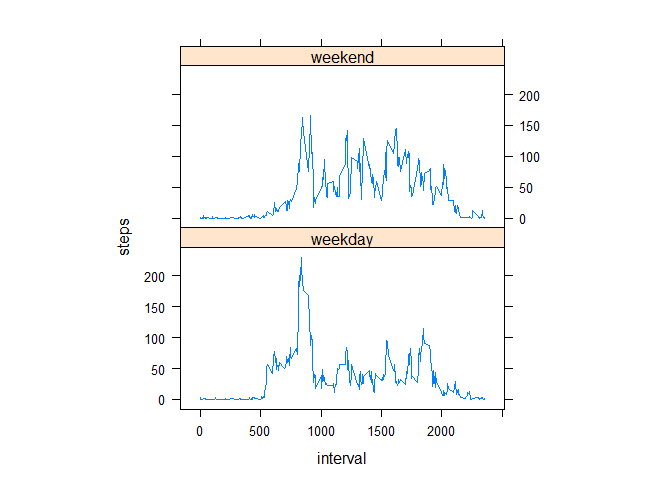
\includegraphics{PA1_template_files/figure-latex/unnamed-chunk-20-1.pdf}

The plots show that there is difference in movement activity between
weekdays and weekends


\end{document}
